\documentclass[12pt]{article}
\usepackage{graphicx}
\usepackage{amssymb}
\usepackage{epstopdf}
\usepackage{amsmath}
\usepackage{multicol}
\usepackage{tcolorbox}
\usepackage{geometry}
\usepackage{enumitem}
\usepackage{fancyhdr}

\DeclareGraphicsRule{.tif}{png}{.png}{`convert #1 `dirname #1`/`basename #1 .tif`.png}

\textwidth = 6.5 in
\textheight = 9 in
\oddsidemargin = 0.0 in
\evensidemargin = 0.0 in
\topmargin = -23pt
\headheight = 0.0 in
\headsep = 0.0 in
\parskip = 0.2in
\parindent = 0.0in
\pagestyle{fancy}
\pagenumbering{gobble}

\newtheorem{theorem}{Theorem}
\newtheorem{corollary}[theorem]{Corollary}
\newtheorem{definition}{Definition}
%\includegraphics [height=50mm, width=50mm]{PathInt.jpg}
\title{Title} 

\begin{document}
%INSTRUCTOR NOTES

 Name:
 \begin{center}\large{5.1 Measuring Distance Traveled}\end{center}

\begin{enumerate}
\item Suppose that an object moving along a straight line path has its velocity in feet per second at time $t$ in seconds given by the graph below.  \\
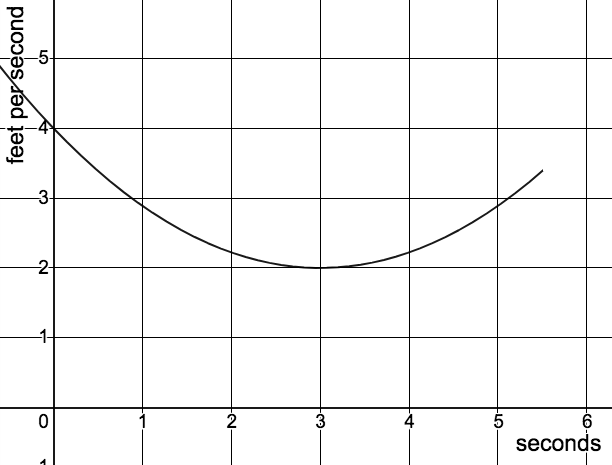
\includegraphics [scale=.3]{5_1_sum}
	\begin{enumerate}
	\item Estimate the distance traveled from $t=2$ to $t=5$.
	\vfill
	\item Use 4 left rectangles to approximate the distance traveled on the interval\\ $2\le t\le5$. How wide is each rectangle?
		\vfill
	\item Use 4 right rectangles to approximate the distance traveled on the interval\\ $2\le t\le5$. How wide is each rectangle?
		\vfill
	\item Suppose the exact value of the velocity is given by the equation $$\displaystyle v\left(t\right)=\frac{2}{9}\left(t-3\right)^{2}+2.$$
Compute the distance traveled on the interval $2\le t\le5$ using a 4 right-rectangle approximation. Show your work. Do you think this is an under or over estimate?
		\vfill
			\vfill
	\end{enumerate}
\newpage
~
\item The graph below gives the vertical velocities of a helicopter drone in meters per second. Positive velocities indicate upward travel, and negative velocities indicate downward travel. \\
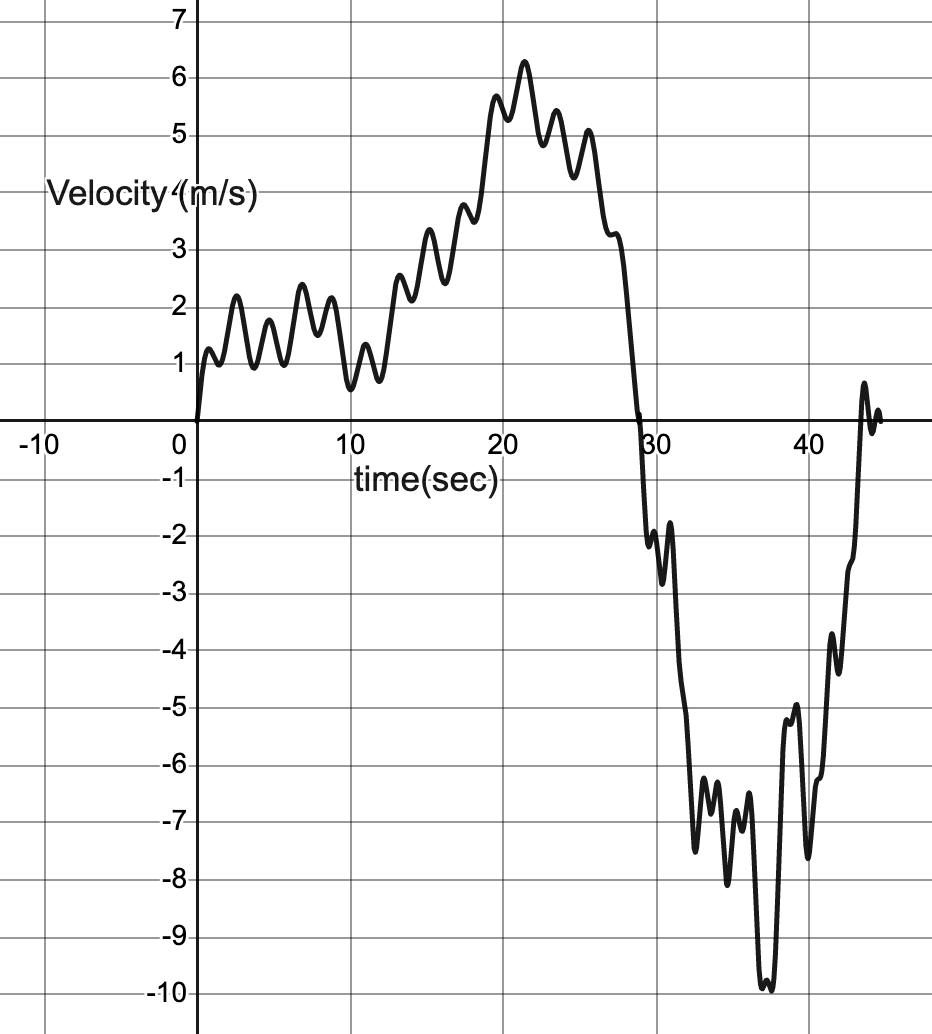
\includegraphics [scale=.2]{5_1_drone}\\
	\begin{enumerate}
	\item When is the drone traveling the fastest? Why?
	\vfill
	\item When is the drone highest in the air? Why?
	\vfill
	\item Estimate the maximum height of the drone. Explain your reasoning.
	\vfill
	\end{enumerate}
\vfill
\item A car comes to a stop five seconds after the driver applies the brakes. While the brakes are on, the velocities in the table are recorded.\\
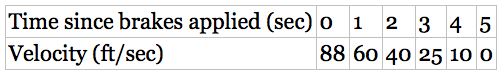
\includegraphics [scale=.5]{5_1_brakes}
	\begin{enumerate}
	\item Give lower and upper estimates of the distance the car traveled after the brakes were applied.
	\vfill
	\item Find the difference between the estimates. How can you explain this difference?
	\end{enumerate}
	\vfill

\end{enumerate}
\end{document}
%%%%%%%%%

\item The following data is gathered as a small plane travels down the runway toward takeoff. How far might the plane travel in the 10 second period? What is an upper estimate? What is a lower estimate? Use the graph below to justify your reasoning.\\
\includegraphics [scale=.5]{5_1_planedata}\\
\includegraphics [scale=.35]{5_1_plane}
\vfill


\item A spin class instructor is designing a 1-hour workout for the stationary bicycle. The graph below shows the speed of the bike (in miles per hour) as a function of time (in minutes).\\
\includegraphics [height=60mm, width=75mm]{5_1_speed}

	\begin{enumerate}
	\item Estimate how many miles (virtual) she traveled. (Be careful of units.) 
	\vfill
	\item How accurate is your estimate? Is it an under or an over estimate? What might you do to make your estimate more accurate? Explain your reasoning.
	\vfill
	\item Sketch a graph of the distance traveled, with total number of miles on the  vertical axis and time in minutes on the horizontal axis. What is the relationship between the graph you drew and the above graph?
		
	\includegraphics [height=60mm, width=75mm]{5_1_blankspeed}
\newpage

\item What are other ways to estimate the distance traveled?\\
\includegraphics [height=60mm, width=75mm]{5_1_speed} \includegraphics [height=60mm, width=75mm]{5_1_speed}
	\end{enumerate}
	\vfill
	
	
\begin{tcolorbox}
\textbf{Warm-up: } Solve the following equations for $t$.
\begin{multicols}{2}
\begin{enumerate}
\item $(t+1)^2=9$
\item $tx+x^2=5$
\end{enumerate}
\end{multicols}
\end{tcolorbox}

MINIPAGE
\noindent\begin{minipage}{0.3\textwidth}% adapt widths of minipages to your needs
try 1
\end{minipage}%
\hspace{40mm}
\begin{minipage}{0.6\textwidth}
a) $f'(2)=$\\\

b) $f'(4)=$\\

c) $f'(6)=$\\

d) $f'(7)=$\\

e) $f'(8)=$
\end{minipage}
